\begin{figure*}[p]
\centering
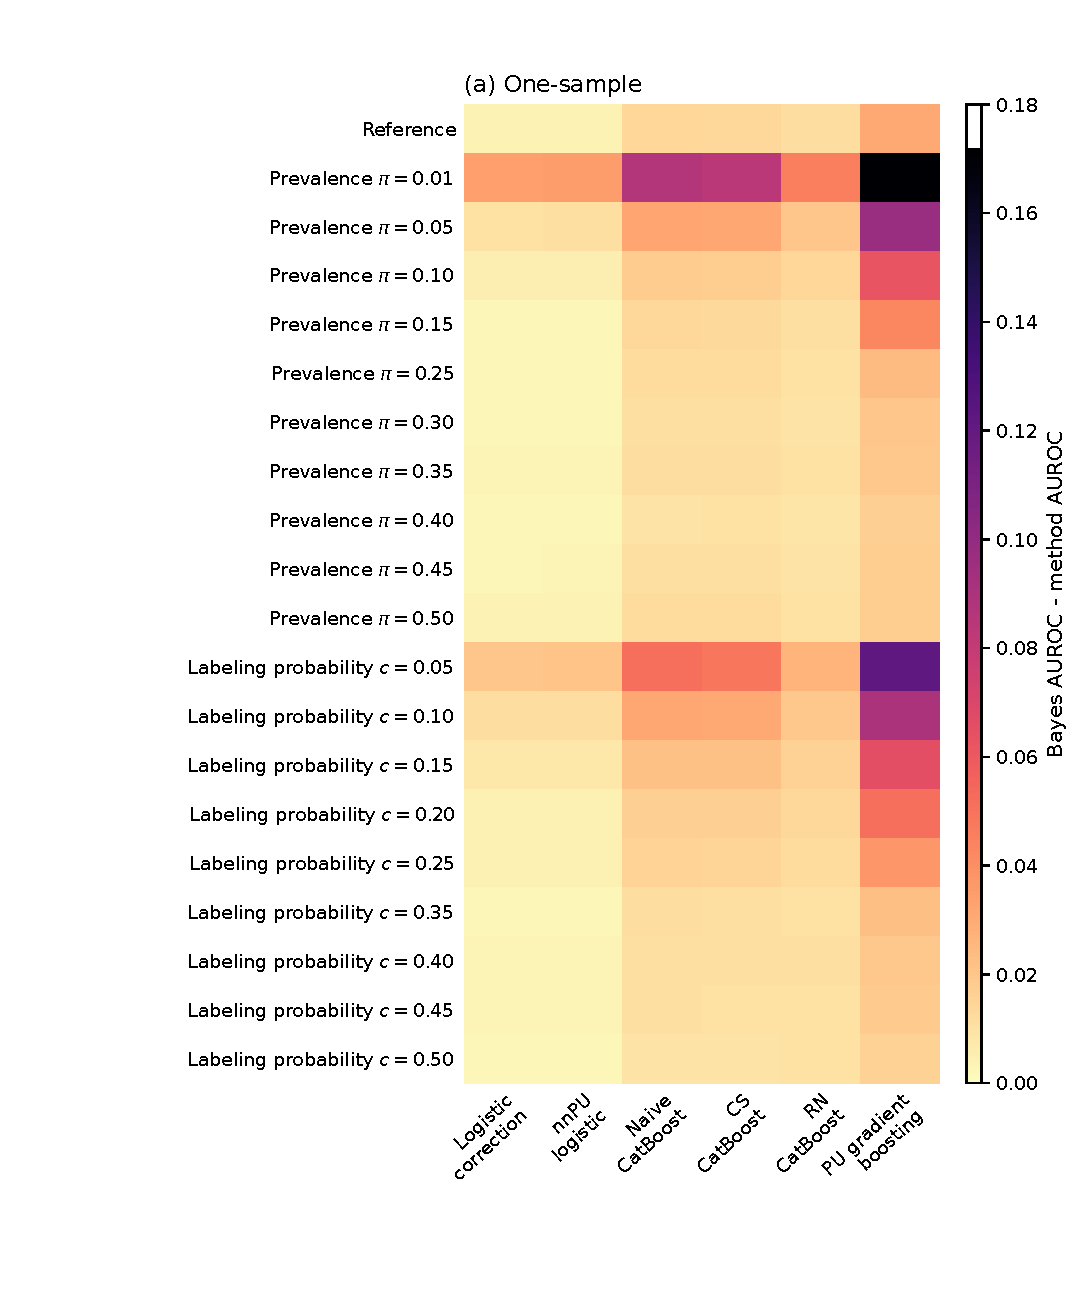
\includegraphics[page=1,width=\textwidth]{revised_figures/fig_s_bayes_regret.pdf}
\caption{Bayes AUROC minus fixed-method AUROC for the six conceptual representatives in all 40 original settings with validated Bayes references. Lower regret is better. One-sample / settings 1--20. All settings retain their validated analytic or exact-likelihood-ratio Bayes reference; lower regret is better.}
\label{fig:s-bayes-regret-1}
\end{figure*}
\begin{figure*}[p]
\centering
\includegraphics[page=2,width=\textwidth]{revised_figures/fig_s_bayes_regret.pdf}
\caption{Bayes AUROC minus fixed-method AUROC for the six conceptual representatives in all 40 original settings with validated Bayes references. Lower regret is better. One-sample / settings 21--40. All settings retain their validated analytic or exact-likelihood-ratio Bayes reference; lower regret is better.}
\label{fig:s-bayes-regret-2}
\end{figure*}
\begin{figure*}[p]
\centering
\includegraphics[page=3,width=\textwidth]{revised_figures/fig_s_bayes_regret.pdf}
\caption{Bayes AUROC minus fixed-method AUROC for the six conceptual representatives in all 40 original settings with validated Bayes references. Lower regret is better. Two-sample / settings 1--20. All settings retain their validated analytic or exact-likelihood-ratio Bayes reference; lower regret is better.}
\label{fig:s-bayes-regret-3}
\end{figure*}
\begin{figure*}[p]
\centering
\includegraphics[page=4,width=\textwidth]{revised_figures/fig_s_bayes_regret.pdf}
\caption{Bayes AUROC minus fixed-method AUROC for the six conceptual representatives in all 40 original settings with validated Bayes references. Lower regret is better. Two-sample / settings 21--40. All settings retain their validated analytic or exact-likelihood-ratio Bayes reference; lower regret is better.}
\label{fig:s-bayes-regret-4}
\end{figure*}
